\subsection{Session page}
To create a session the user must first reach the Sessions component, which can be accessed through the “Sessions” button on the navbar. The session page has the URL /admin/sessions. A session cannot be created until a course is present in the database. Therefore, the user needs to visit the Dashboard site first, before accessing the session page. The figure \ref{fig:sessionPage} shows the session page, in this figure two sessions have already been created called “% TODO write session name %”
\\[11pt]
The Session component is visible in the Sessions component on the right side of the page. The Sessions component contains a search bar and a select element identical to the ones on the question page. The component also contains a list that includes all the current sessions for the chosen course. Like in the list on the question page, the list on the session page must send a socket message to the server in order to keep its session list updated. The list is updated whenever the Sessions component is loaded, a new session is created, or whenever the chosen course is changed. If there are no sessions for the chosen course, then only the Sessions component is displayed on the page with no entries in the session list.
\\[11pt]
Once the Session component is visible, the information displayed in the component varies depending on the selected question. The user can easily change between the available sessions and their questions by clicking on them. On figure \ref{fig:sessionPage} it is shown see that the session “% Session Name %” has opened the question “% Question Title %”. 
\\[11pt]
The Session component uses the DisplayQuestion component to display the question information. The DisplayQuestion is a component that is used to show question information, question solution, and student answers. The DisplayQuestion component is used on several pages, including the session page and the user profile page. The DisplayQuestion component uses the b-tabs element, which makes it easier to toggle between showing the question information and the question solution. There is a component for the answer object and a component for the solution object for each question type in the DisplayQuestion component. Only one of these can be used at the same time. The DisplayQuestion component must accommodate for the fact that some of the question types require the GraphDrawer to display their solution object. The DisplayQuestion component needs to display the shown question type. This is done to avoid confusing users with certain question types, as some of the question types have a similar format in the GraphDrawer. When the DisplayQuestion component is used in the Sessions component, the admin or student assistant can mark an incorrect answer as correct. The DisplayQuestion component only shows incorrect answers, except when it is used on the user profile page.
\begin{figure}[H]
    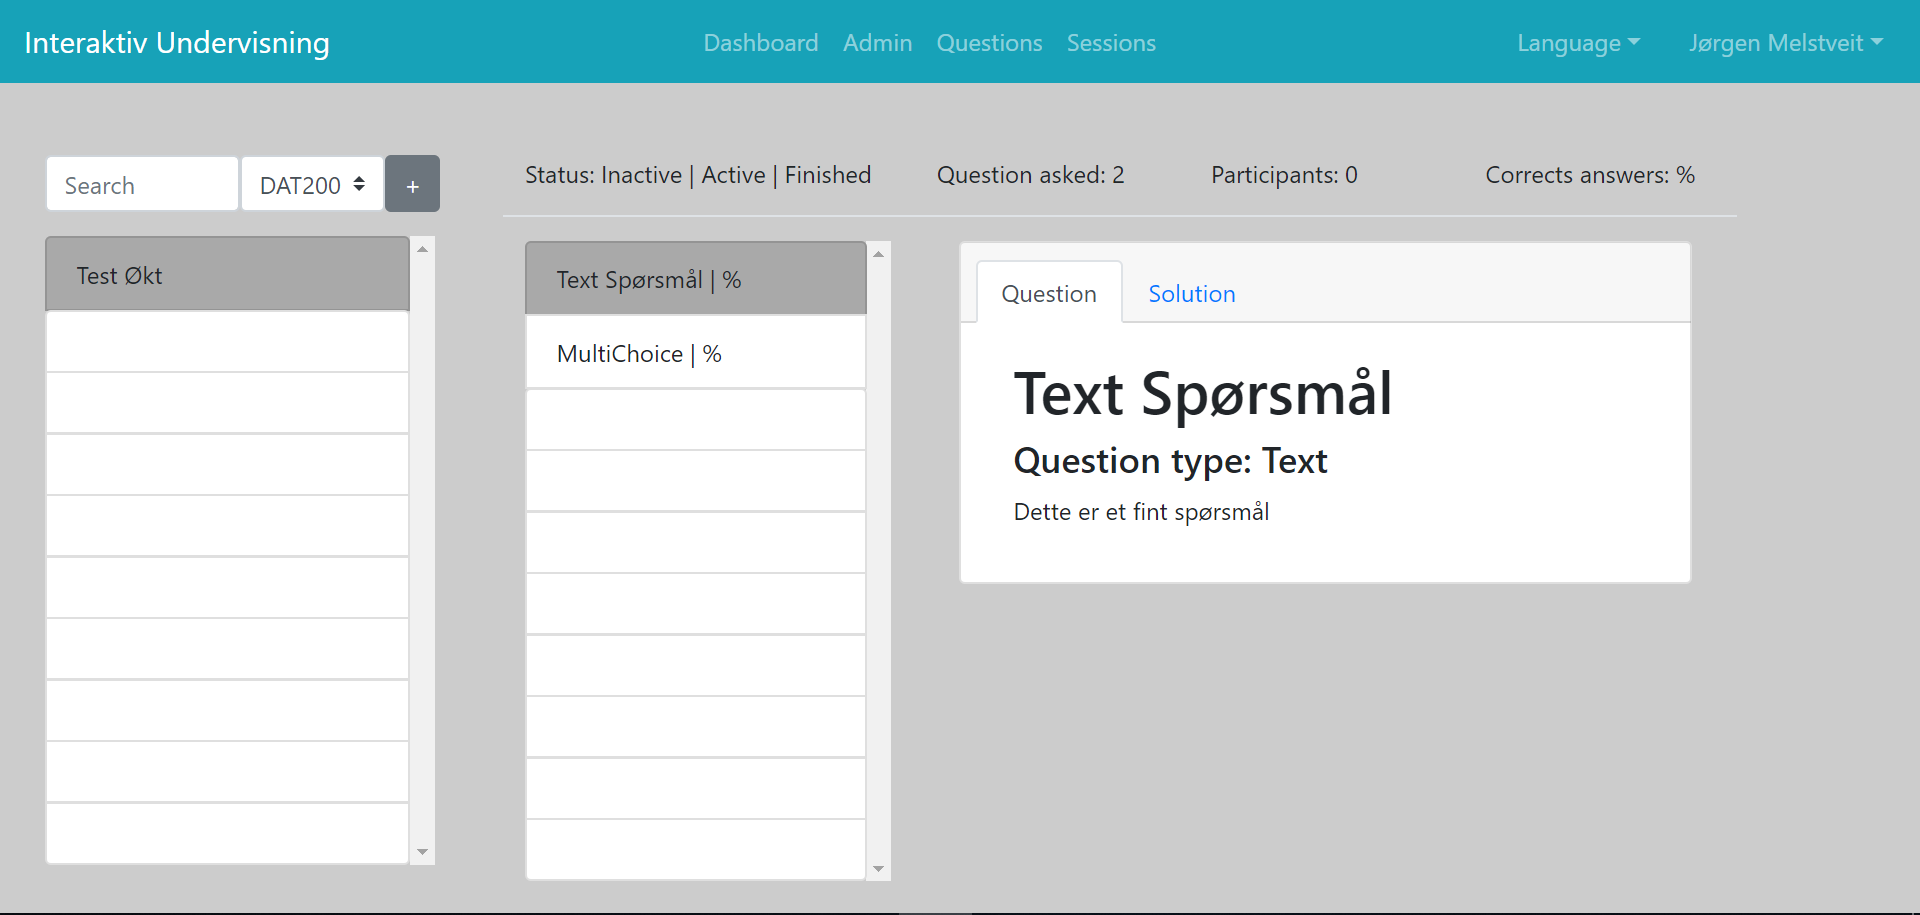
\includegraphics[width=0.80\linewidth]{sessionPage}
    \caption{This figure displays the session page. In the image, the user is currently checking out the session %Insert Session Name%. The Session and DisplayQuestion components are both visible to the right of the image. Currently, the % Insert question title % is selected, and the DisplayQuestion component is showing its basic information.
    }
    \label{fig:sessionPage}
\end{figure}
\noindent
To create a new session, the EditSession component must first be opened. This is done by having the user click on the "+" button.
This component displays all the available questions of the chosen course using a Bootstrap modal. Like the EditQuestion component, the EditSession component has a data property object called \code{newSession}. This object should have all the values needed for the server to create a new session and add it to the database. The current course should have already been chosen at this point, therefore the course variable in the \code{newSession} object has been assigned with this course value. This value is used by EditSession component whenever it sends a socket message to the server, asking the server for all the questions in the given course. The EditSession component allows the user to give the session a title and add a question to the session. Once a user has chosen one of the questions, the question is added to the questions array in the \code{newSession} object. The content of the questions array is displayed in the EditSession component under the previous list. If the content of the questions array is changed, the list is automatically updated. This is noticeable in the figure \ref{fig:editSessionComponent}, where you can see the %Insert text title% has been added to the list under the questions list. Once a question is visible in this way, it means the question is a part of the newly created session. Of course, nothing is stored on the server until the user has confirmed its changes with the “Ok” button. When the button is pressed the EditQuestion sends a socket message with the \code{newSession} object to the server. The server retrieves the information from the \code{newSession} object, and it is used to insert a new session into the Session database table. Afterward, all the questions in the questions array are linked to the session in the SessionsHasQuestion database table. When the session has been added, the server sends a response back to the client. The EditSession component should be closed and the Sessions component reacts to the response by sending a new request back to the server, requesting an updated session list. Once the server responds with the updated session content, the list on the Session component should include the newly created session.  
\begin{figure}[H]
    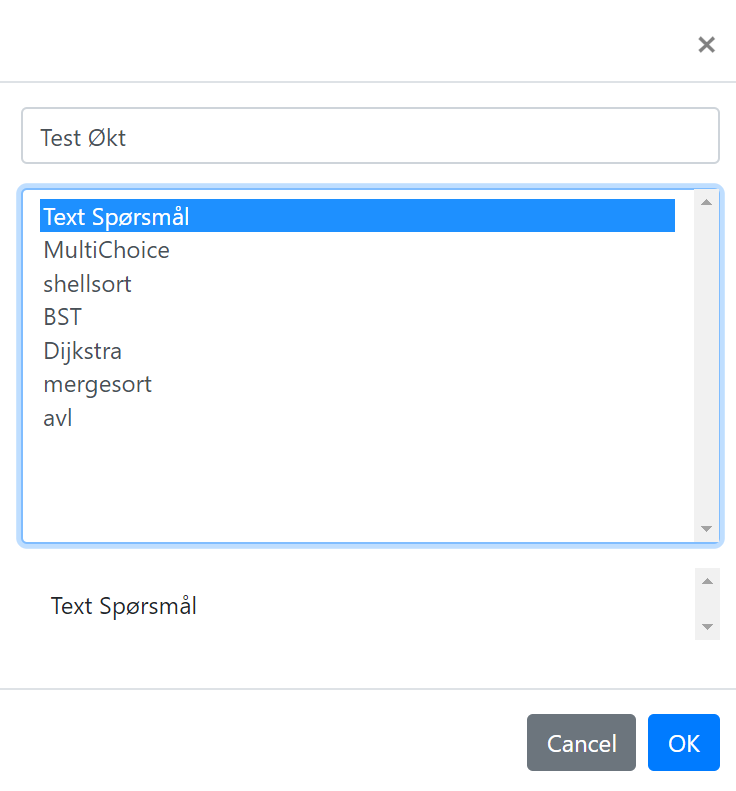
\includegraphics[width=0.80\linewidth]{createANewSession}
    \caption{This figure displays an image of the EditSession component. In the image, the user is planning on creating a new session by the name of %Insert session name%. The image also shows the user having clicked on the %Insert question title%, which now have been added to the list at the bottom of the page.
    }
    \label{fig:editSessionComponent}
\end{figure}
\noindent
It is also possible to edit or delete existing sessions, but only if their status is set to “Inactive”. The session status is visible on the Session component, where the current session status is the status that is visibly underlined. The status will remain “Inactive” as long as it is not initialized. When an admin or student assistant starts a waiting room for a session. The status changes to “Active”, and it is no longer possible to edit or delete this session. Once a session is finished and all the questions have been answered, the status is changed to “Finished”. If an admin user or student assistant decides to use this session again, then the status is changed back to “Active” again until the session is finished. The reason for not allowing any users to edit or delete active sessions are the same for not allowing users the ability to edit or delete questions once they’ve been assigned to a session. Deleting or editing a session after use would affect the previous session results for both the teacher and students. If the status is no longer “Inactive” the background color to the edit and the delete buttons are changed to gray. This is an indication that these buttons are no longer to be used. If a user still tries to click on the buttons, the user is informed that it is no longer possible to use this functionality. Using the edit functionality works similarly as it did for the editing questions. The EditQuestion component is again used, but all the data previously saved for the chosen session are filled in the component. Any changes done to the session will not apply until the user confirms their action using the button labeled “OK”. On the server side, the server will update the session title, then remove all links with questions, then create new links with the updated question list. Removing a session simply sends a socket request to the server asking the server to delete the selected session from the database. After the session is deleted from the database, the list in the Sessions component is updated again, and the selected session should no longer be visible on the page.
